\section{Proposed SCL Framework}\label{sec:method}

\scl{} is a small, rule-based layer that runs once per frame between the detector and the tracker
(Fig.~\ref{fig:arch}). It groups the scores of recent frames (Sect.~\ref{sec:calib}), decides
whether they are clean or noisy (Sect.~\ref{sec:regimes}), acts on this decision, and can pass a
weak candidate that clearly continues a track (Sect.~\ref{sec:rescue}). The detector and the
tracker are never changed.

In short, a detection travels through \scl{} as follows. Its score is turned into a logit and
compared with two splits computed from the scores of the last 10 frames: below the first split it
is background, between the splits uncertain, and above the second confident. If most recent
foreground scores are confident, the stream is clean and the detection reaches the tracker with
its own score. Otherwise the stream is noisy: a background detection is dropped, and the others
get new scores that tell the tracker whether they may start a track or only continue one. A weak
detection that lies on a track of the previous frame can still be passed on. The tracker then
does its own matching as usual. Its score enters the statistics only after the decision for its
frame.

\begin{figure*}[t]
\centering
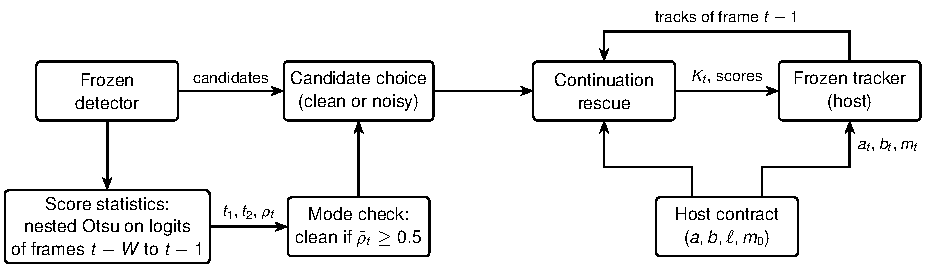
\includegraphics{Fig1.pdf}
\caption{\scl{} between a frozen detector and a frozen tracker (the host). Boxes are processing
steps and arrows show what each step passes on. The score statistics use earlier frames only. The
host contract holds the tracker's published settings. The tracker receives the chosen candidates
$K_t$, their scores, and its thresholds $a_t$, $b_t$ and tolerance $m_t$ for the frame}
\label{fig:arch}
\end{figure*}

\subsection{Inputs and outputs}\label{sec:problem}
In each frame $t$, the detector gives candidates $D_t=\{(\mathbf{x}_i,s_i,c_i)\}$, each with a box
$\mathbf{x}_i$, a score $s_i\in(0,1)$, and a class $c_i$. The layer works on the logit
\begin{equation}
z_i=\log\frac{s_i}{1-s_i},
\label{eq:logit}
\end{equation}
the log-odds transformation of the confidence score. It converts a score between 0 and 1 into a
value on an unrestricted scale while preserving the ordering of scores: a score of 0.5 gives
$z_i=0$, 0.9 gives about $2.2$, and 0.1 about $-2.2$. The logistic function
$\sigma(z)=1/(1+e^{-z})$ turns a logit back into a score. The layer uses logits for two reasons.
Detector scores crowd near 0 and 1, where small differences in score are large differences in
confidence; the logit spreads these regions out, so the histogram splits of
Sect.~\ref{sec:calib} separate the groups more clearly. And a common change of a detector's
scores, a change of temperature, divides all logits by the same number, a simple stretch that the
splits follow (Sect.~\ref{sec:calib}). The host gives its contract $h=(a,b,\ell,m_0)$: the score $a$ needed to match a
track, the score $b$ needed to start one, the lowest score $\ell$ it uses, and its matching
tolerance $m_0$, one minus the smallest intersection over union (IoU) of two boxes that counts as a
match. A single-stage tracker has $\ell=\min(a,b)$, a two-stage tracker $\ell<\min(a,b)$. In
every frame the layer returns
\begin{equation}
\left(K_t,\tilde{s},a_t,b_t,m_t\right)=
\mathcal{L}\left(Z_{<t},D_t,\mathcal{T}_{t-1},g_t;\,h\right):
\label{eq:layer}
\end{equation}
the candidates $K_t$ for the tracker, their scores, and its thresholds and tolerance, from the
logits $Z_{<t}$ of earlier frames, the tracks $\mathcal{T}_{t-1}$, and a camera-motion measure
$g_t$; no future frame is used.

\subsection{Self-calibration from detector scores}\label{sec:calib}
The layer collects the logits $Z_t^W$ of the candidates of the last $W=10$ frames and splits them
twice with Otsu's method \cite{otsu1979}. The first split, $t_1$, separates background (low
logits) from foreground; the second, $t_2$, found on the foreground only, divides it into uncertain
and confident candidates. The share of confident candidates in the foreground,
\begin{equation}
\rho_t=\frac{\left|\{z\in Z_t^W: z\ge t_2\}\right|}{\left|\{z\in Z_t^W: z\ge t_1\}\right|},
\label{eq:rho}
\end{equation}
describes the shape of the score distribution and needs no labels: if 30 of 40 foreground
candidates are confident, $\rho_t=0.75$. Otsu's method is used because it picks a split from the
data alone, without labels or tuning, and applying it twice gives the three groups that one
threshold cannot. For example, for the scores 0.02, 0.03, 0.05, 0.4, 0.5, 0.9, and 0.95 (logits
$-3.9$, $-3.5$, $-2.9$, $-0.4$, 0, 2.2, and 2.9), the first split separates the three lowest scores
as background, and the second divides the other four into 0.4 and 0.5 (uncertain) and 0.9 and 0.95
(confident), so $\rho_t=2/4=0.5$. Because the splits are made on logits, they move with the
scores when the whole logit scale is stretched or shifted, and each group keeps the same
candidates. Figure~\ref{fig:groups} shows the groups for a clean and a noisy stream. When a
detector emits very few low scores, the first split falls inside the objects; since clutter
usually gives more candidates than the objects do, a window with fewer candidates below $t_1$ than
above it counts as clean, $\rho_t=1$ (background check).

\begin{figure}[t]
\centering
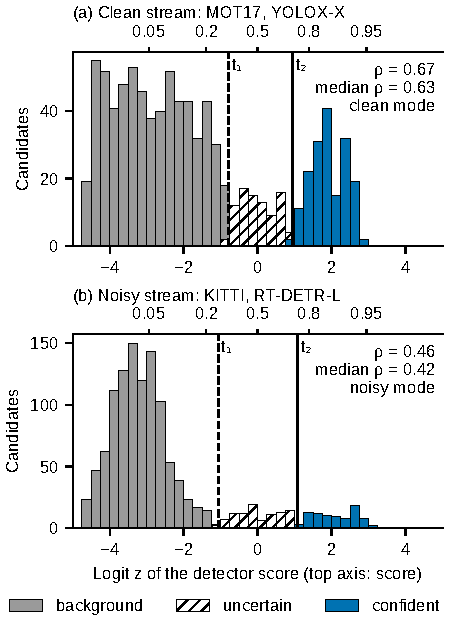
\includegraphics{Fig2.pdf}
\caption{What the layer sees: the logits of the candidates of the last 10 frames, just before its
decision for frame 101, with the Otsu splits $t_1$ (dashed line) and $t_2$ (solid line). Plain
light bars: background; hatched bars: uncertain; plain dark bars: confident. The top axis gives the
matching detector score. (a) MOT17-02 with YOLOX-X: most foreground candidates are confident, and
the stream is clean. (b) KITTI 0001 with RT-DETR-L: many are uncertain, and the stream is noisy.
Values of the frozen layer in the runs of Sect.~\ref{sec:results}}
\label{fig:groups}
\end{figure}

\subsection{Clean and noisy modes}\label{sec:regimes}
Clean and noisy describe the distribution of the scores, not whether a single detection is
correct. The stream is clean at frame $t$ if the median of all $\rho$ values so far is at least one half,
a majority rule, and noisy otherwise; before the first valid split it is cold. Because the median
covers the whole stream, a short drop in confidence does not change the mode, and during
development this whole-stream rule removed mode changes in the middle of streams that had lowered
HOTA (Sect.~\ref{sec:steps}). The splits themselves use only the last $W$ frames, so the groups, and
in the clean mode the threshold cap of Eq.~\eqref{eq:clean}, follow a change of the score scale
within $W$ frames even while the mode stays the same.

\emph{Cold and clean modes.} The tracker keeps its own thresholds and scores, and only cross-class
duplicates are removed. In the clean mode, a threshold so high that it would reject the confident
group is lowered to the score $\sigma(t_2)$ at which that group begins:
\begin{equation}
a_t=\min\!\left(a,\sigma(t_2)\right),\qquad b_t=\min\!\left(b,\sigma(t_2)\right).
\label{eq:clean}
\end{equation}
The clean mode is thus a minimal intervention rather than a plain pass-through: the scores are
kept, and the output equals that of the host alone whenever the confident group lies above the
host's thresholds and no rescue applies, as for BoostTrack, ByteTrack at floor 0.1, and Hybrid-SORT
on MOT17 (Sect.~\ref{sec:results}). When the scores are halved, for example, no score is above 0.5, and ByteTrack in
its official setting ($a=0.6$, $b=0.7$) never starts a track; the splits move with the halved
scores, so Eq.~\eqref{eq:clean} lets the confident candidates reach it again.

\emph{Noisy mode.} Confident candidates ($z\ge t_2$) may start and continue tracks, uncertain ones
($t_1\le z<t_2$) may only continue tracks, and background candidates are dropped. Each score is
replaced by its mid-rank $u_i\in(0,1)$ among the scores of a remap memory, which stores the scores
kept in the first frame and in every 10th frame, the last 20 of them (tied scores share their average
rank, and before the first sample the current frame is used),
\begin{equation}
\tilde{s}_i=
\begin{cases}
0.5+0.5\,u_i, & z_i\ge t_2,\\
0.1+0.4\,u_i, & t_1\le z_i<t_2,
\end{cases}
\label{eq:remap}
\end{equation}
and both thresholds are set to $a_t=b_t=0.5$, so uncertain candidates can only reach a tracker's
low-score step. A weaker candidate that overlaps a stronger one with IoU above one half is removed,
unless a different track of the previous frame claims it, which keeps people who stand close
together in a crowd.

\subsection{Track continuation and camera motion}\label{sec:rescue}
A track can be lost when its object gets low scores for a few frames, above all in single-stage
trackers, which have no low-score step. The rescue passes such a candidate, with its score raised
just above the lowest threshold of the frame, when it is in the foreground (or, for a
single-stage tracker, when there is no background group), overlaps a track of the previous frame
with IoU of at least one half, no other usable candidate covers that track, and the tracker could
not see it otherwise. It thus gives single-stage trackers the continuation step they lack. The
rescue only makes the box visible; the tracker itself still decides, with its own matching,
whether and to which track it is assigned.

In noisy frames, the matching tolerance also grows with camera motion. The motion is the shift
between consecutive grayscale frames at quarter resolution, found by phase correlation
\cite{reddy1996phasecorr}, and $r_t$ is its ratio to its median over the last 100 frames ($r_t=1$
during a warm-up of 5 frames or if this median is zero):
\begin{equation}
m_t=\min\!\left(0.95,\;1-\frac{1-m_0}{\max(1,r_t)}\right).
\label{eq:motion}
\end{equation}
With $m_0=0.8$ and twice the usual motion, a match needs an IoU of 0.1 instead of 0.2.

\subsection{Host contract and adapters}\label{sec:contract}
Table~\ref{tab:contracts} lists the contracts; each value is taken from the tracker's published
configuration, and none is fitted. For each tracker family, a small adapter writes the layer's
candidates, scores, thresholds, and tolerance into the tracker's existing parameters before each
update and then calls the tracker's own update. The matching steps, motion model, track
management, and any post-processing of the authors run unchanged, so the host stays frozen: its
code, weights, and association algorithm do not change, only the values of its thresholds are set
for each frame, and the rules are the same for every tracker.

\begin{table}[t]
\caption{Host contracts: the published settings of each tracker, as used by the layer: matching
(association) threshold $a$, birth threshold $b$, low threshold $\ell$, and match tolerance $m_0$.
For every tracker, the layer's decision is passed on as thresholds, candidates, and scores.}
\label{tab:contracts}
\centering\footnotesize
\setlength{\tabcolsep}{4pt}
\begin{tabular}{@{}>{\raggedright\arraybackslash}p{27mm}lcccc@{}}
\toprule
Tracker (setting) & Type & $a$ & $b$ & $\ell$ & $m_0$\\
\midrule
ByteTrack (official MOT17) & two-stage & 0.6 & 0.7 & 0.1 & 0.8\\
ByteTrack (library default) & two-stage & 0.25 & 0.25 & 0.1 & 0.8\\
BoT-SORT (library default) & two-stage & 0.25 & 0.25 & 0.1 & 0.8\\
SparseTrack & two-stage & 0.6 & 0.7 & 0.1 & 0.85\\
BoostTrack & two-stage & 0.6 & 0.6 & 0.1 & 0.7\\
Hybrid-SORT & two-stage & 0.6 & 0.6 & 0.1 & 0.75\\
OC-SORT & single-stage & 0.6 & 0.6 & 0.6 & 0.7\\
PD-SORT & single-stage & 0.6 & 0.6 & 0.6 & 0.7\\
\bottomrule
\end{tabular}
\end{table}


\subsection{Parameter values}\label{sec:constants}
Table~\ref{tab:constants} lists all values of \scl{}. They were fixed before the external
evaluation, are the same for every tracker, detector, and dataset, and none was chosen by searching
over a range of values. They come from standard values (the IoU of 0.5 of MOT evaluation and the
common thresholds 0.5 and 0.1), from definitions, and from design choices kept fixed in all
development stages. Algorithm~\ref{alg:layer} summarizes the steps for one frame.

\begin{table}[t]
\caption{Values of \scl{} and their source.}
\label{tab:constants}
\centering\footnotesize
\setlength{\tabcolsep}{3pt}
\begin{tabular}{@{}>{\raggedright\arraybackslash}p{19mm}>{\raggedright\arraybackslash}p{27mm}>{\raggedright\arraybackslash}p{25mm}@{}}
\toprule
Value & Setting & Source\\
\midrule
Window $W$ & 10 frames & design choice\\
Mode rule & clean if median $\rho\ge0.5$ & majority rule\\
Background check & $\rho=1$ if fewer below $t_1$ than above & rule: no background group\\
Noisy score ranges & $[0.5,1)$, $[0.1,0.5)$ & common thresholds\\
Noisy $a_t$, $b_t$ & 0.5 & common threshold\\
Remap memory & 20 frames, one every 10 & design choice\\
Duplicate, rescue IoU & 0.5 & MOT evaluation IoU\\
Rescued score & lowest threshold $+\,0.001$ & just above the threshold\\
Motion cue & phase correlation, quarter resolution & standard method \cite{reddy1996phasecorr}\\
Motion history & 100 frames, warm-up 5 & design choice\\
Tolerance cap & 0.95 & minimum overlap 0.05\\
\bottomrule
\end{tabular}
\end{table}


\begin{algorithm}[t]
\caption{\scl{} for frame $t$. The window holds the logits of frames
$t-W$ to $t-1$, so the decision for frame $t$ uses no future frame.}\label{alg:layer}
\begin{algorithmic}[1]
\Require candidates $D_t$, tracks $\mathcal{T}_{t-1}$, motion cue $g_t$, contract $(a,b,\ell,m_0)$, constants of Table~\ref{tab:constants}
\Ensure candidates $K_t$, scores $\tilde{s}$, thresholds $a_t,b_t$, tolerance $m_t$
\State $z_i\gets$ logit of $s_i$ for all $i$ \Comment{Eq.~\eqref{eq:logit}}
\If{no valid split exists} \Comment{e.g., first frame}
  \State mode $\gets$ cold; $(a_t,b_t)\gets(a,b)$
\Else
  \State $(t_1,t_2)\gets$ nested Otsu on the window \Comment{Sect.~\ref{sec:calib}}
  \State $\rho_t\gets$ Eq.~\eqref{eq:rho} with the background check
  \State mode $\gets$ clean if $\mathrm{median}(\rho)\ge0.5$, else noisy
\EndIf
\If{mode is cold or clean} \Comment{Sect.~\ref{sec:regimes}}
  \State remove cross-class duplicates; keep raw scores
  \If{clean} set $(a_t,b_t)$ by Eq.~\eqref{eq:clean}
  \EndIf
\Else \Comment{noisy mode}
  \State remove duplicates with track context
  \State drop $z<t_1$; remap scores by Eq.~\eqref{eq:remap}
  \State $a_t\gets0.5$; $b_t\gets0.5$
\EndIf
\State rescue continuations (not cold) \Comment{Sect.~\ref{sec:rescue}}
\State $m_t\gets$ Eq.~\eqref{eq:motion} if noisy, else $m_0$
\State pass $K_t$, $\tilde{s}$, $a_t$, $b_t$, $m_t$ to the tracker
\State add the logits left after duplicate removal to the window
\State add $g_t$ to the motion history
\State store the tracks of frame $t$ after the tracker update
\end{algorithmic}
\end{algorithm}
